\chapter{Vorlesung}
Ohne Beweis (siehe später Edmonds-Krap-Algorithmus) gilt:\\
Die Zeit der Schichten im Levelnetzgraph des Hopcraft-Karp-Algorithmus steigt mindestens um eins von Durchlauf zu Durchlauf.
\[ |M^*|-|M|\leq\footnote{Lemma von Berge} \frac{|V|}{k}~~~~\tilde{G}=(V_1\cup V_2, M\oplus M^*) \]
$k$ Mindestlänge der $M$-augm. Pfade
\paragraph{Ziel}
Laufzeit von Hopcraft-Karp $=\mathcal{O}(\sqrt{|V|}\cdot|E|)$
\subparagraph{1. Phase}
$k$ Schleifendurchläufe $\Rightarrow$ Danach haben $M$-augm. Pfade mindestens die Länge $k$
\subparagraph{2. Phase}
Weitere $\frac{|V|}{k}$ Schleifendurchläufe genügen, um zum Maximum-Matching $M^*$ zu gelangen.
\subsection{Gesamtzahl der Schleifendurchläufe}
\[ S(k)=k+\frac{|V|}{k}~~S'(k)=1-\frac{|V|}{k^2}=0\Rightarrow k=\sqrt{|V|} \]
$\Rightarrow$ Zahl der Schleifendurchläufe $\leq \sqrt{|V|}$
\section{Algorithmen zur Berechnung maximaler Flüsse}
\begin{wrapfigure}{l}{0.4\linewidth}
	\centering
	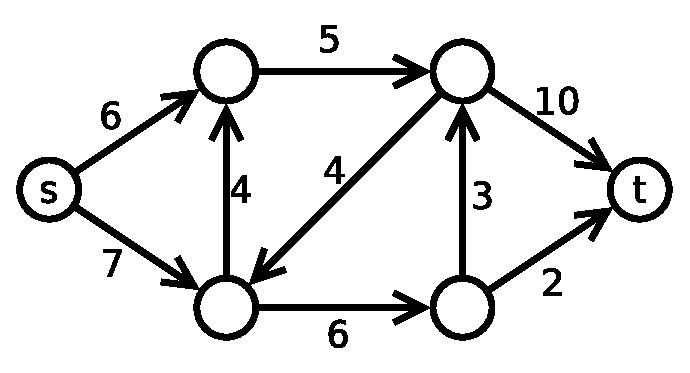
\includegraphics[width=\linewidth]{24/Grafik/Diagramm1}
	\caption{...}
	\label{fig:1}
\end{wrapfigure}
$ $
\[ c\footnote{Kapazität}:E\rightarrow\mathbb{R}^+_0 \]
Gesucht:
\[ f:E\rightarrow\mathbb{R}^+_0 \]
\[ \forall (u,v)\in E : \text{Kapazitätsbedingung: } 0\leq f(u,v)\leq c(u,v) \]
\pagebreak
\subsection{Flusserhaltung}
\begin{wrapfigure}{l}{0.3\linewidth}
	\centering
	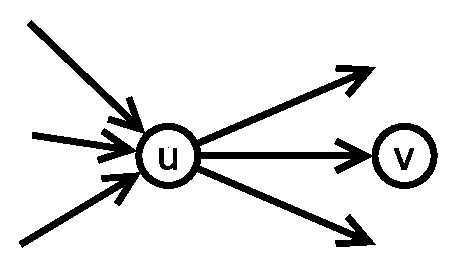
\includegraphics[width=\linewidth]{24/Grafik/Diagramm2}
	\caption{...}
	\label{fig:2}
	\end{wrapfigure}
	$ $
\[ \forall u\in V\setminus\{ s,t \} \]
\[  \underset{\text{Fluss aus $u$ herraus}}{\underbrace{\sum_{v\in V} f(u,v)}} = \underset{\text{Fluss in $u$ herein}}{\underbrace{\sum_{v\in V} f(v,u)}}  \]
\[ (u,v) \notin E \Rightarrow c(u,v) = 0 \Rightarrow f(u,v) = 0 \]
\[ (u,v) \in E \Rightarrow (v,u) \notin E~~~\text{Konventionen} \]
\begin{figure}[H]
\centering
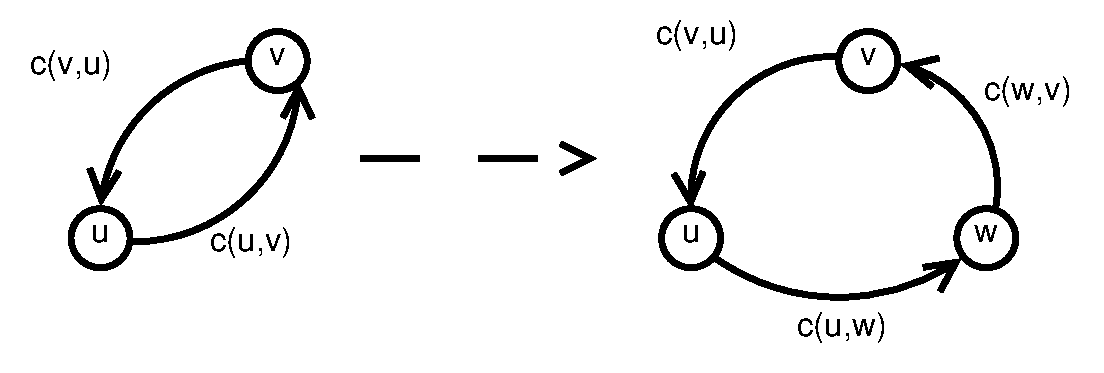
\includegraphics[width=0.7\linewidth]{24/Grafik/Diagramm3}
\caption{...}
\label{fig:Diagramm3}
\end{figure}
\begin{figure}[H]
	\centering
	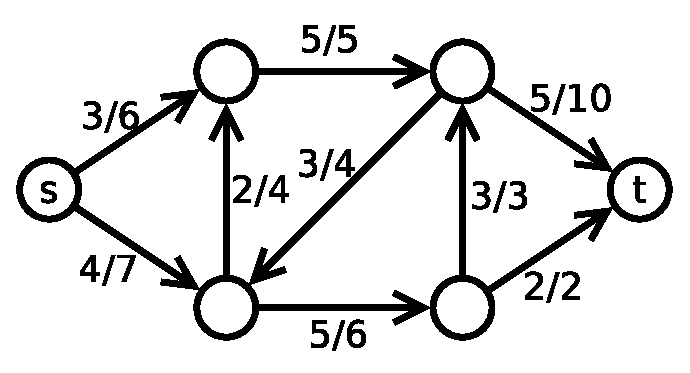
\includegraphics[width=0.7\linewidth]{24/Grafik/Diagramm4}
	\caption{Beispiel für einen Fluss}
	\label{fig:Diagramm4}
\end{figure}


\subsection{Definition}
$|f| \hat{=}$ Fluss, der von $s$ nach $t$ transportiert wird.
\[ |f| = \sum_{v\in V} f(s,v) - \sum_{v\in V} f(v,s) = \sum_{v\in V} f(v,t) - \sum_{v\in V} f(t,v) \]
\paragraph{Gesucht:} maximaler Fluss $|f|$
\pagebreak
\subsection{Definition: Schnitt $(S,T)$}
\begin{wrapfigure}{l}{0.5\linewidth}
	\centering
	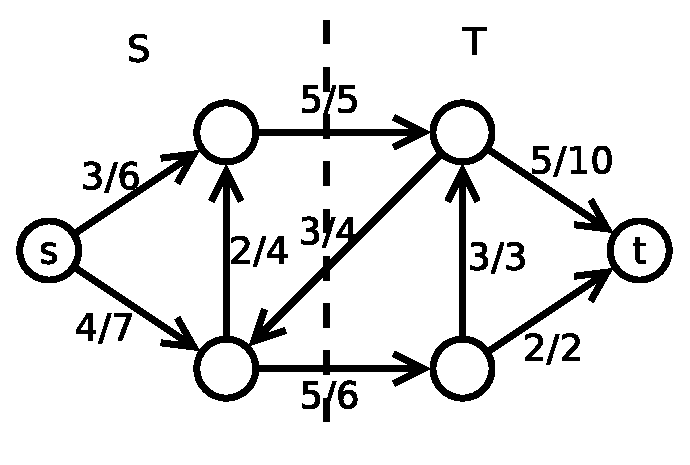
\includegraphics[width=\linewidth]{24/Grafik/Diagramm5}
	\caption{Beispiel Schnitt}
	\label{fig:Diagramm5}
\end{wrapfigure}
$ $
\[ S\dot{\cup} T = V~~ s\in S, t\in T \]
\subsubsection{Schnittkapazität}
\[ \sum_{u\in S}\sum_{v\in T} c(u,v) = c(S,T) \]
\subsubsection{Fluss über Schnitt}
\[ \sum_{u\in S}\sum_{v\in T} f(u,v) - \sum_{u\in S}\sum_{v\in T} f(v,u) \leq c(S,T) \]
\vspace{40pt}
\[ |f| = \sum_{v\in V} f(s,v) - \sum_{v \in V}f(v,s)+\overset{=0}{\overbrace{\sum_{u\in S\setminus\{ s \}} \left( \sum_{v\in V} f(u,v) - \sum_{v \in V} f(v,u) \right)   }} = \sum_{u \in S} \left(\sum_{v\in V}f(u,v)-\sum_{v \in V}f(v,u)   \right) \]
\[ =\sum_{u \in S}\left(  \sum_{v\in S} f(u,v)+\sum_{v\in T}f(u,v) - \sum_{v \in S}f(v,u)- \sum_{v\in T}f(v,u)  \right) \]
\[ \left( \sum_{u\in S}\sum_{v\in T} f(u,v) -\sum_{u\in S}\sum_{v\in T} f(v,u)  \right) + \overset{=0}{\overbrace{\left(  \sum_{u\in S}\sum_{v\in S}f(u,v) - \sum_{u\in S}\sum_{v\in S} f(v,u) \right)} } = f(S,T)\]
\subsection{Konstruktion des Restnetzwerk $G_f$}
\begin{figure}[H]
\centering
\begin{subfigure}[H]{0.3\linewidth}
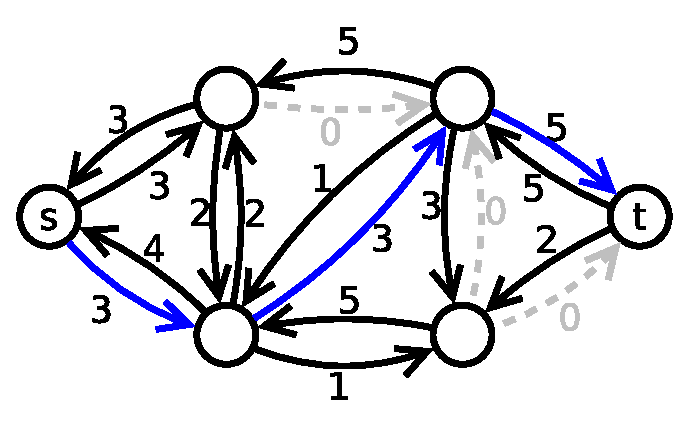
\includegraphics[width=\linewidth]{24/Grafik/Diagramm6}
\caption{Restnetzwerk zum Graphen \ref{fig:Diagramm4}}
\end{subfigure}
\begin{subfigure}[H]{0.3\linewidth}
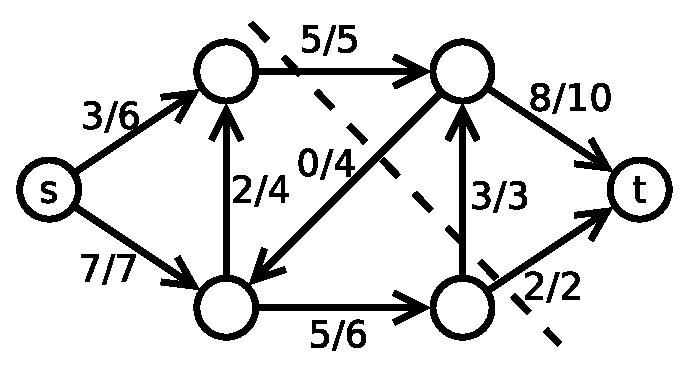
\includegraphics[width=\linewidth]{24/Grafik/Diagramm7}
\caption{Mit Restnetzwerk optimierter Graph}
\end{subfigure}	
\label{fig:Diagramm6}
\end{figure}
\[ |f| = f(S,T) \leq c(S,T) \]
\section{Ford-Fulkerson-Algorithmus}
\begin{lstlisting}
f = 0;
do {
	p = flussverbessernder Pfad im Restnetzwerk $G_f$;
	$c_{min}$ = kleinste Restkapazität der kanten von p;
	erhöhe den Fluss $f$ entlang von p um $c_min$
} while (p $\neq$ NULL);
\end{lstlisting}